\documentclass[a4paper,12pt]{article}
\usepackage[utf8]{inputenc}
\usepackage{geometry}
\geometry{a4paper, margin=1in}
\usepackage{hyperref}
\usepackage{amsmath}
\usepackage{enumitem}
\usepackage{titlesec}
\usepackage{fancyhdr}
\usepackage{parskip}
\usepackage{tikz}
\usetikzlibrary{shapes, arrows.meta, positioning}

% Header and footer
\pagestyle{fancy}
\fancyhf{}
\fancyhead[L]{Basketball Scoring System Using ESP32}
\fancyhead[R]{\today}
\fancyfoot[C]{\thepage}

% Section formatting
\titleformat{\section}{\Large\bfseries}{\thesection}{1em}{}
\titleformat{\subsection}{\bfseries}{\thesubsection}{1em}{}

% TikZ styles
\tikzset{
  block/.style={rectangle, draw, rounded corners, minimum width=3cm, minimum height=1cm, text centered, fill=blue!20},
  io/.style={trapezium, trapezium left angle=70, trapezium right angle=110, minimum width=3cm, minimum height=1cm, text centered, draw, fill=green!20},
  arrow/.style={-{Latex[length=3mm]}, thick},
  cloud/.style={ellipse, draw, fill=red!20, minimum height=1cm, text centered}
}

\begin{document}

\begin{center}
    {\LARGE \textbf{Real-Time Basketball Scoring System Using ESP32}}\\[0.5em]
    \textbf{Project Procedure and Design Document}\\[1em]
    \today
\end{center}

\hrule
\vspace{1em}

\section{Project Overview}

This document details the complete procedure to build a \textbf{real-time basketball scoring and player stats tracking system} using an \textbf{ESP32 microcontroller}. The system supports tracking scores, fouls, assists, rebounds, steals, game clock management, and displays live updates on a Smart TV and control panel accessible via web browsers over Wi-Fi.

\vspace{1em}
\noindent \textbf{Key Features:}
\begin{itemize}[noitemsep]
    \item Team score and foul tracking
    \item Player-level statistics (points, fouls, assists, rebounds, steals)
    \item Game clock with start, pause, reset, and quarter control
    \item Real-time updates via WebSocket communication
    \item Web-based scoreboard (for Smart TV) and control panel (for mobile devices)
    \item Physical buttons input integrated with web control input
\end{itemize}

\section{Hardware Setup}

\subsection{Components Required}
\begin{itemize}[noitemsep]
    \item ESP32 development board (Wi-Fi enabled)
    \item Physical push buttons for input (score increments, fouls, clock control, player selection)
    \item Pull-up or pull-down resistors (typically 10 k$\Omega$)
    \item Breadboard and jumper wires or custom PCB
    \item Optional: OLED display for debugging/local display
    \item Wi-Fi router or use ESP32 Access Point mode for standalone operation
\end{itemize}

\subsection{Button Assignments}
Map physical buttons to following functions (example):
\begin{itemize}[noitemsep]
    \item Team A and Team B score increments (+1, +2, +3 points)
    \item Team fouls increment
    \item Game clock controls (start, pause, reset)
    \item Player selection (via buttons or rotary encoder)
    \item Player stat increments (fouls, assists, rebounds, steals)
\end{itemize}

\section{Software Architecture}

\subsection{ESP32 Firmware Responsibilities}
\begin{itemize}[noitemsep]
    \item Manage physical button inputs using GPIO and interrupts or polling
    \item Maintain internal game state: team scores, fouls, player stats, and game clock
    \item Host a web server with WebSocket support to:
    \begin{itemize}[noitemsep]
        \item Serve scoreboard and control panel web pages stored in SPIFFS/LittleFS
        \item Send real-time game state updates to connected clients
        \item Receive control commands from web clients
    \end{itemize}
    \item Synchronize game state across all connected clients and hardware inputs
\end{itemize}

\subsection{Data Structures}

Define a player data structure to track full stats:

\begin{verbatim}
struct Player {
    String name;
    int number;
    int points;
    int fouls;
    int assists;
    int rebounds;
    int steals;
    bool onCourt;
};
\end{verbatim}

Use arrays or vectors for team rosters (limit 10-12 players/team).

\section{Networking and Communication}

\subsection{Wi-Fi Modes}
\begin{itemize}[noitemsep]
    \item \textbf{Access Point Mode:} ESP32 creates its own Wi-Fi network to which Smart TV and control devices connect.
    \item \textbf{Station Mode:} ESP32 connects to an existing Wi-Fi network shared with Smart TV and control devices.
\end{itemize}

\subsection{Communication Protocol}
\begin{itemize}[noitemsep]
    \item Use WebSockets (e.g., via AsyncWebSocket library) for bidirectional real-time communication.
    \item ESP32 broadcasts game state updates as JSON to all connected clients.
    \item Clients send control commands (stat updates, clock control) to ESP32.
\end{itemize}

\section{Web Interface Design}

\subsection{Scoreboard Page}
\begin{itemize}[noitemsep]
    \item Large, clear display optimized for Smart TV screens
    \item Shows team scores, fouls, current quarter, and game clock
    \item Displays player stats: points, fouls, assists, rebounds, steals
    \item Scrollable or paginated roster display for each team
    \item Auto-updates on receiving WebSocket data
\end{itemize}

\subsection{Control Panel Page}
\begin{itemize}[noitemsep]
    \item Touch-friendly interface for mobile devices
    \item Player selection controls (dropdown or numeric input)
    \item Buttons to increment stats (points, fouls, assists, rebounds, steals)
    \item Game clock controls: start, pause, reset, quarter change
    \item Sends commands via WebSocket to ESP32
\end{itemize}

\section{Game Clock Management}

\begin{itemize}[noitemsep]
    \item Use \texttt{millis()} timer in ESP32 to track elapsed game time
    \item Support start, pause, reset, and quarter transitions
    \item Periodically broadcast clock updates to connected clients
\end{itemize}

\section{Data Persistence and Export (Optional)}

\begin{itemize}[noitemsep]
    \item Store current game stats in SPIFFS/LittleFS as JSON or CSV files
    \item Allow exporting match summaries for post-game analysis
    \item Limit data retention due to ESP32 memory constraints
\end{itemize}

\section{Integration and Testing}

\begin{enumerate}[label=\arabic*.]
    \item Test physical button input and debouncing
    \item Verify ESP32 Wi-Fi connection and web server availability
    \item Load scoreboard and control panel on devices and test real-time updates
    \item Test synchronization between physical inputs and web commands
    \item Simulate a full game flow including player stat updates and clock management
    \item Perform stress test with multiple clients connected simultaneously
\end{enumerate}

\section{Project Enhancements (Future Work)}

\begin{itemize}[noitemsep]
    \item Add audio feedback (buzzers) for game events
    \item Implement OTA (Over-the-Air) firmware updates
    \item Integrate with external databases or cloud services for long-term storage
    \item Enhance UI with team logos, colors, and animations
    \item Implement player substitution and lineup management
\end{itemize}

\section*{Summary of Skills Demonstrated}

\begin{tabular}{ll}
\textbf{Category} & \textbf{Skills} \\
\hline
Embedded Systems & GPIO handling, interrupts, timers, memory management \\
Networking & Wi-Fi setup, HTTP server, WebSocket protocol \\
Software Development & C++ programming, JSON handling, file system (SPIFFS) \\
Web Development & HTML, CSS, JavaScript, responsive UI, WebSocket client \\
Systems Integration & Multi-device real-time communication and synchronization \\
User Experience & Touch UI design, scalable display layout for TV and mobile \\
\end{tabular}

\vspace{2em}

\section{System Architecture Diagram}

\begin{center}
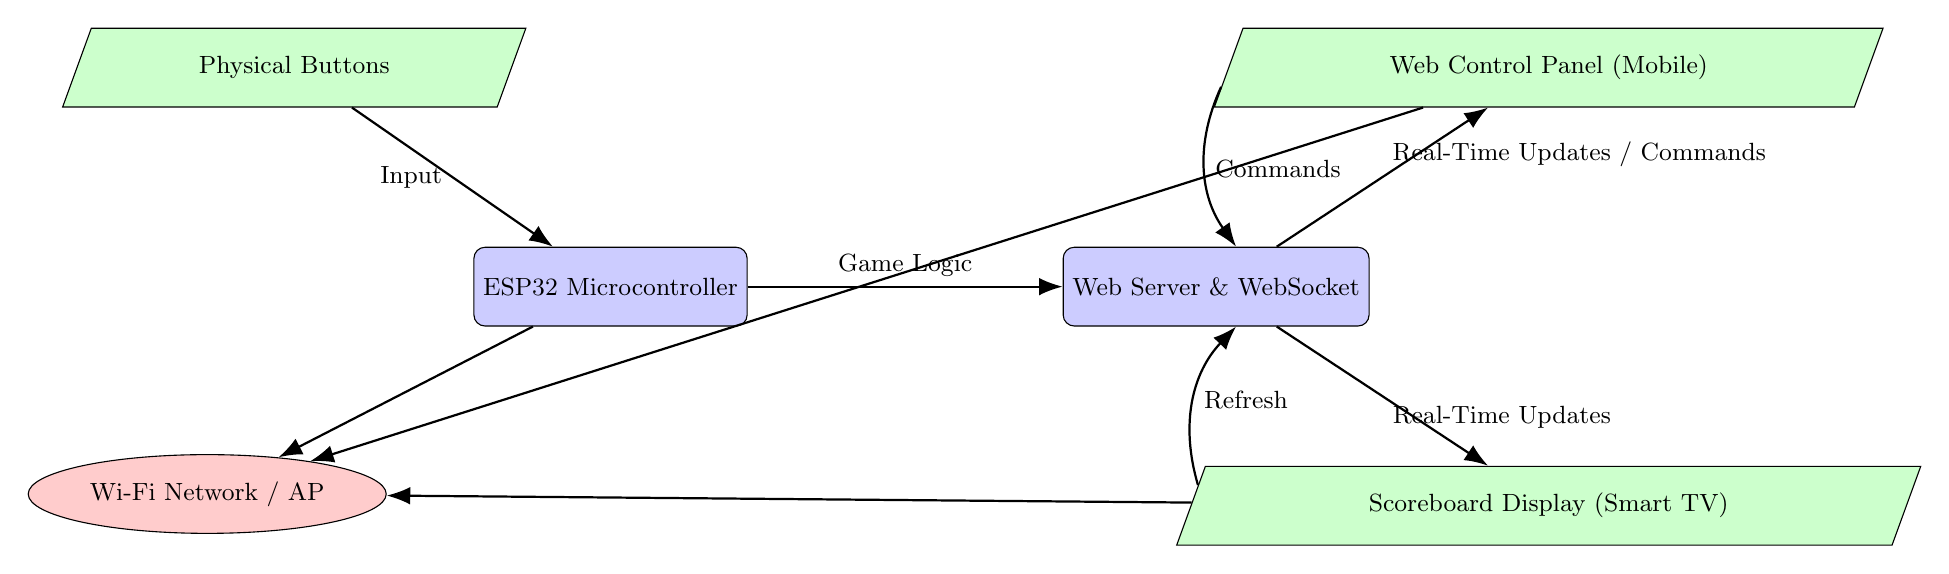
\begin{tikzpicture}[node distance=2.5cm, every node/.style={font=\small}]
  % Nodes
  \node[block] (esp32) {ESP32 Microcontroller};
  \node[io, above left=of esp32] (buttons) {Physical Buttons};
  \node[block, right=4cm of esp32] (webserver) {Web Server \& WebSocket};
  \node[io, above right=of webserver] (controlpanel) {Web Control Panel (Mobile)};
  \node[io, below right=of webserver] (scoreboard) {Scoreboard Display (Smart TV)};
  \node[cloud, below left=of esp32] (wifi) {Wi-Fi Network / AP};
  
  % Connections
  \draw[arrow] (buttons) -- (esp32) node[midway, left] {Input};
  \draw[arrow] (esp32) -- (webserver) node[midway, above] {Game Logic};
  \draw[arrow] (webserver) -- (controlpanel) node[midway, above right] {Real-Time Updates / Commands};
  \draw[arrow] (webserver) -- (scoreboard) node[midway, below right] {Real-Time Updates};
  \draw[arrow, bend right] (controlpanel) to node[midway, right] {Commands} (webserver);
  \draw[arrow, bend left] (scoreboard) to node[midway, right] {Refresh} (webserver);
  \draw[arrow] (esp32) -- (wifi);
  \draw[arrow] (controlpanel) -- (wifi);
  \draw[arrow] (scoreboard) -- (wifi);
\end{tikzpicture}
\end{center}

\section{Data Flow Diagram}

\begin{center}
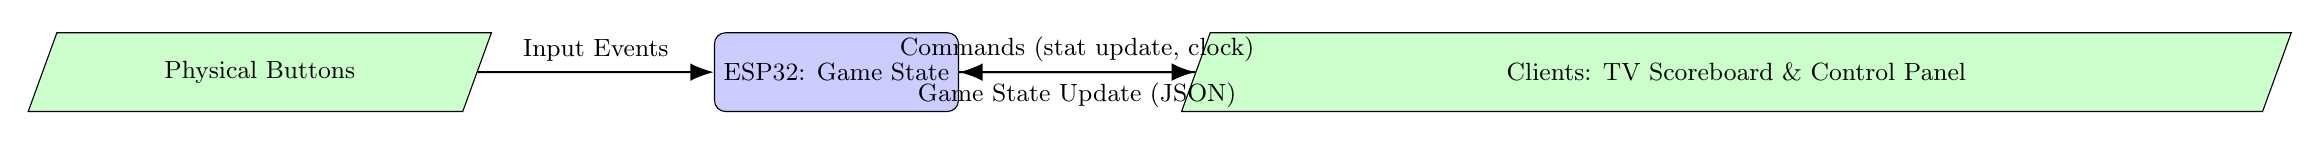
\begin{tikzpicture}[node distance=3cm, every node/.style={font=\small}]
  % Nodes
  \node[block] (esp32) {ESP32: Game State};
  \node[io, left=of esp32] (buttons) {Physical Buttons};
  \node[io, right=of esp32] (clients) {Clients: TV Scoreboard \& Control Panel};
  
  % Connections
  \draw[arrow] (buttons) -- (esp32) node[midway, above] {Input Events};
  \draw[arrow] (clients) -- (esp32) node[midway, above] {Commands (stat update, clock)};
  \draw[arrow] (esp32) -- (clients) node[midway, below] {Game State Update (JSON)};
\end{tikzpicture}
\end{center}

\vspace{2em}

\hrule
\vspace{1em}

\begin{center}
    \textit{This document serves as a complete guideline for developing a real-time basketball scoring and player stats system using ESP32, blending embedded and web technologies for a professional, industry-relevant project.}
\end{center}

\end{document}
